\documentclass[compress]{beamer}
\usepackage[
    title={Markowitz e CAPM: Analisi Empirica su Orizzonti Multipli},
    subtitle={Valutazione empirica del modello di Markowitz su orizzonti temporali multipli con test dell'ipotesi del CAPM},
    event={Progetto fine corso MPSMF},
    author={L. Falasca},
    longauthor={Luca Falasca},
    email={luca.falasca@students.uniroma2.eu},
    institute={Tor Vergata},
    longinstitute={Università degli Studi di Roma Tor Vergata},
]{unislides}
\usepackage{graphicx} % Required for inserting images
\usepackage{minted}
\usepackage{algorithm}
\usepackage{hyperref}
\usepackage{adjustbox}
\usepackage{svg}
\svgsetup{inkscapelatex=false}

\begin{document}

\begin{frame}[plain]
	\titlepage
\end{frame}
\section{Introduzione}

\subsection{Obiettivi}
\begin{frame}{\subsecname}
	\begin{itemize}
		\item Valutazione su base empirica del modello di Markowitz
		\item Analisi su diversi orizzonti temporali
		      \begin{itemize}
			      \item Giornaliero
			      \item Settimanale
			      \item Mensile
		      \end{itemize}
		\item Stazionarietà
		\item Portafoglio tangente
		\item Capital market line
		\item CAPM hypotesys test
		\begin{itemize}
			\item Portafoglio di mercato
			\item Portafoglio equamente pesato
		\end{itemize}
	\end{itemize}

\end{frame}

\subsection{Dati e risorse tecniche}
\begin{frame}{\subsecname}
	\begin{itemize}
		\item Il progetto è stato realizzato in Python
		\item I dati sono stati prelevati da Yahoo Finance e da Federal Reserve Bank of St. Louis
	\end{itemize}
	\vspace{0.5cm}
	\begin{minipage}{0.3\textwidth}
		\centering
		
\includegraphics[width=0.5\linewidth]{images/Python-logo.png}
	\end{minipage}
	\begin{minipage}{0.3\textwidth}
		\centering
		
\includegraphics[width=0.7\linewidth]{images/Yahoo!_Finance_logo.png}
	\end{minipage}
	\begin{minipage}{0.3\textwidth}
		\centering
		\includesvg[width=1.2\linewidth]{images/FRB-STL-WEB-blue-gold.svg}
	\end{minipage}
\end{frame}

\section{Markowitz Model}

\subsection{Tassi di rendimento}
\begin{frame}{\subsecname}
	Per stimare la volatilità $\sigma$ del tasso di rendimento $r_T$ dello stock $S$, dobbiamo ricorrere ai dati storici sullo stock. Sfruttiamo i prezzi di chiusura dello stock per un ampio intervallo di tempo passato. Denotiamo con

	\[
		S_1, S_2, \dots, S_N, S_{N+1},
	\]

	le variabili aleatorie la cui realizzazione ha dato luogo al prezzo di chiusura dello stock nell'$n$-simo giorno di contrattazione per $n = 1, \dots, N+1$, dove $N+1$ è il numero di giorni di mercato del trascorso anno di riferimento. Formalmente, il tasso di rendimento dello stock a termine dell’$n+1$-simo giorno di contrattazione, inteso come variabile aleatoria, è definito come

	\[
		r_n \overset{\text{def}}{=} \frac{S_{n+1} - S_n}{S_n}, \quad \forall n = 1, \dots, N,
	\]
\end{frame}
\begin{frame}{\subsecname}
	Nel caso giornaliero verrà utilizzato il tasso di rendimento logaritmico, perché approssima in maniera adeguata quello reale

	\[
		\rho_n \overset{\text{def}}{=} \log \left( \frac{S_{n+1}}{S_n} \right), \quad \forall n = 1, \dots, N.
	\]

    Invece nei casi settimanali e mensili dovremmo usare il tasso di rendimento classico definito precedentemente
\end{frame}

\subsection{Stazionarietà}
\begin{frame}{\subsecname}
	Possiamo osservare la stazionarietà del processo dei tassi di rendimento che cambia a seconda del periodo temporale considerato. 
	\begin{minipage}{0.49\textwidth}
		\centering
		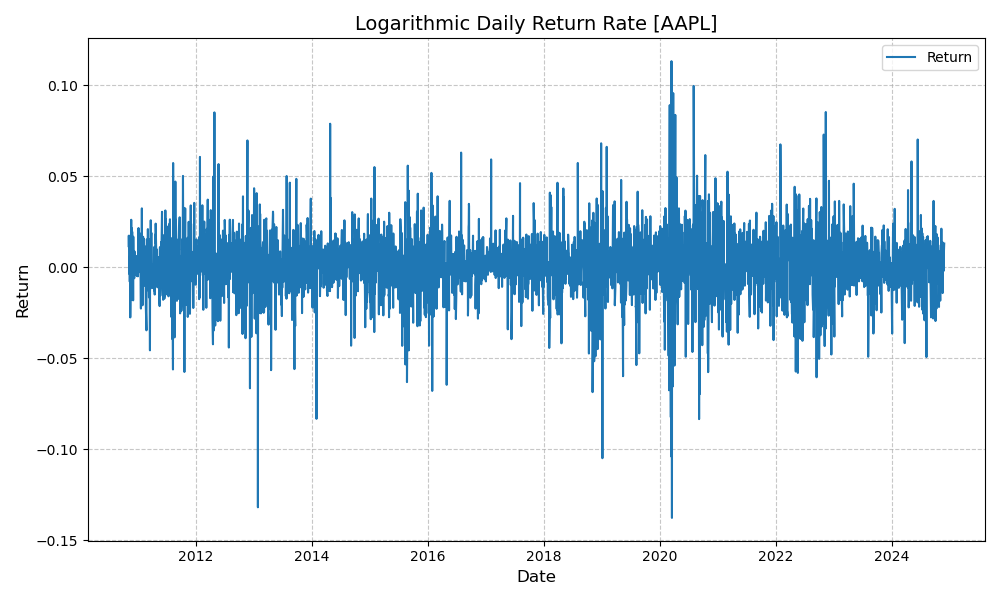
\includegraphics[width=0.8\linewidth]{images/Logarithmic Daily Return Rate [AAPL].png}
	\end{minipage}
	\hfill
	\begin{minipage}{0.49\textwidth}
		\centering
		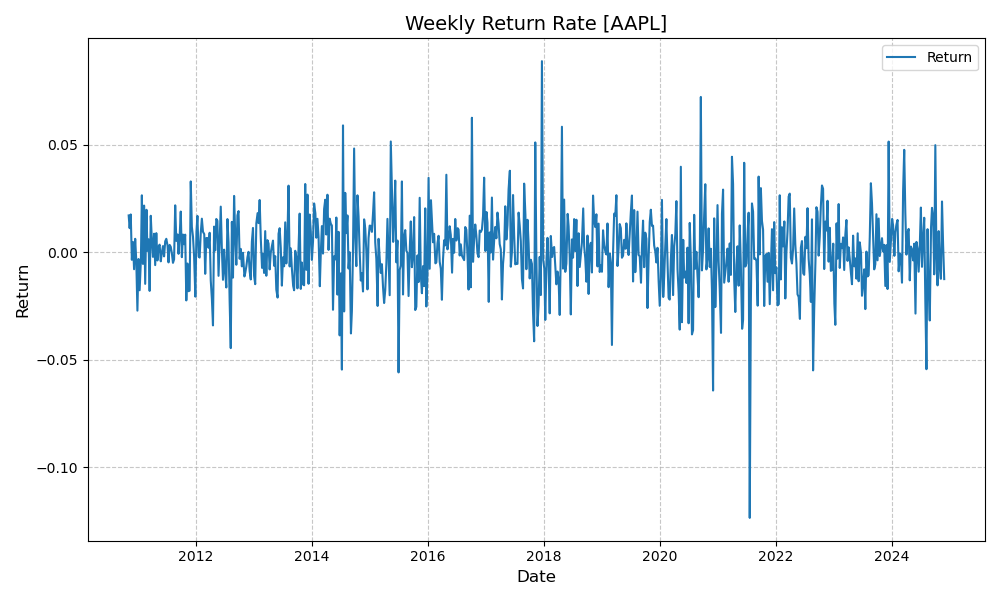
\includegraphics[width=0.8\linewidth]{images/Weekly Return Rate [AAPL].png}
	\end{minipage}
	\vspace{-0.5cm}
	\begin{center}
		\begin{minipage}{0.5\textwidth}
			\centering
			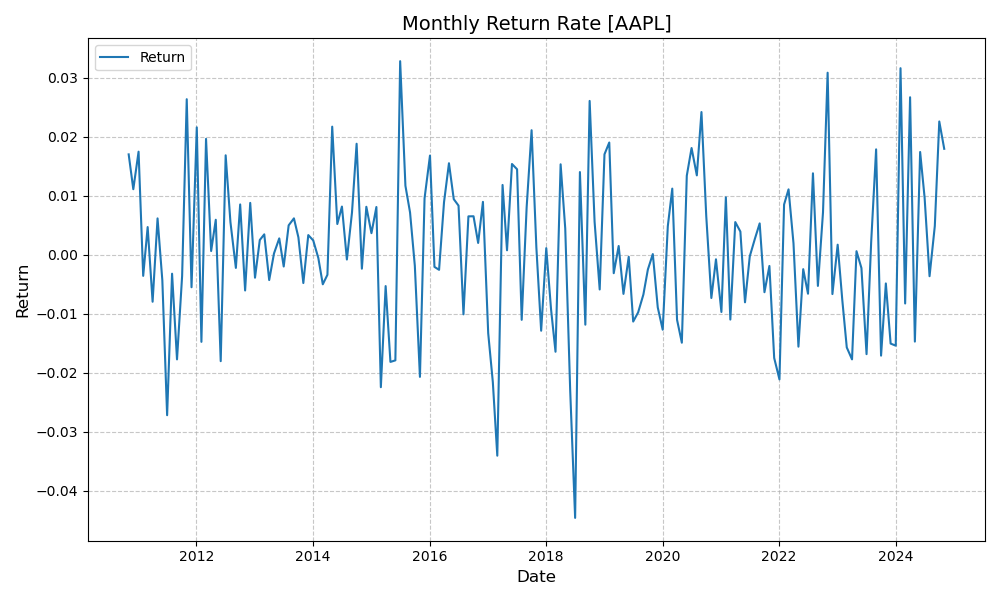
\includegraphics[width=0.8\linewidth]{images/Monthly Return Rate [AAPL].png}
		\end{minipage}
	\end{center}
\end{frame}

\subsection{Autocorrelazione}
\begin{frame}{\subsecname}
	Questo fenomeno è osservabile anche tramite l'autocorrelazione parziale
	\begin{minipage}{1\textwidth}
		\centering
		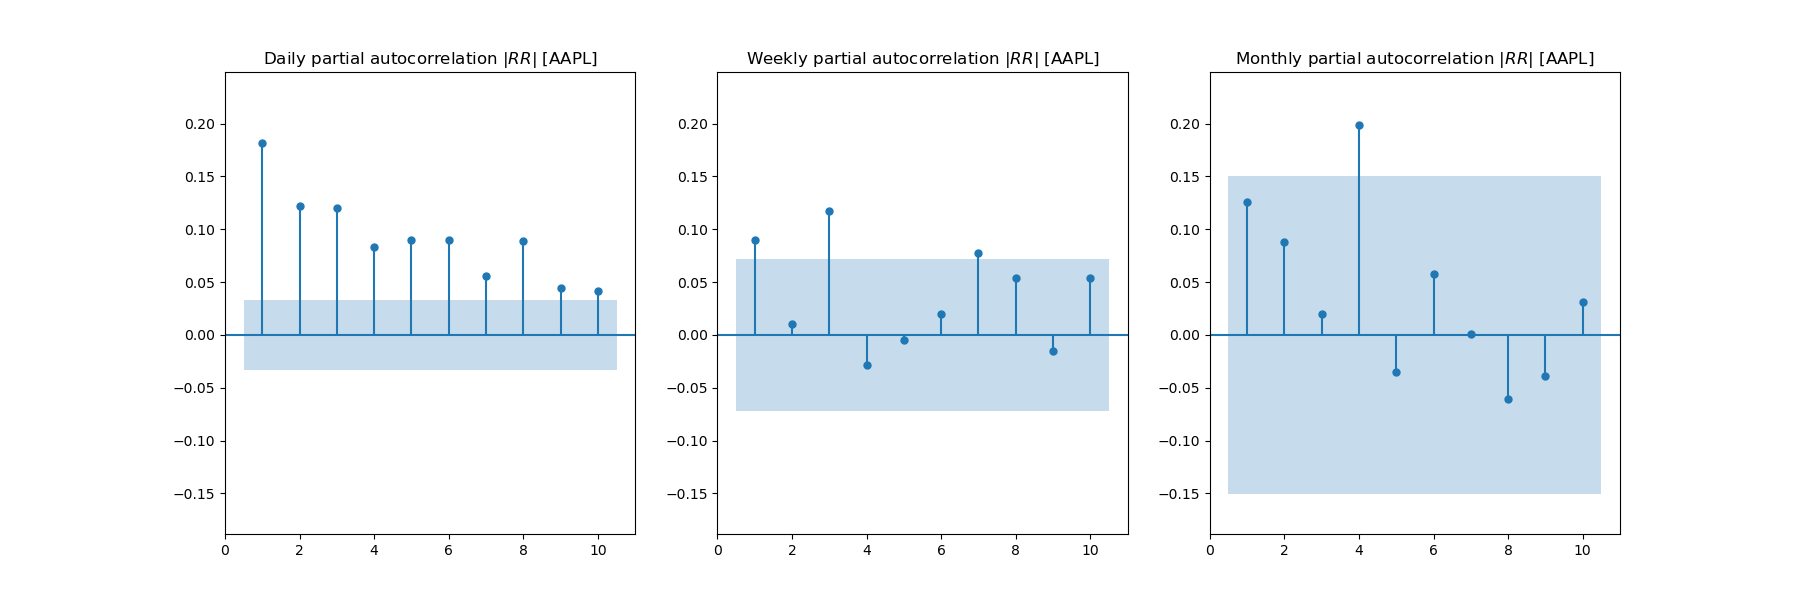
\includegraphics[width=0.8\linewidth]{images/partial_autocorrelation_abs_AAPL.png}
	\end{minipage}
	\vspace{-0.5cm}
	\begin{minipage}{1\textwidth}
		\centering
		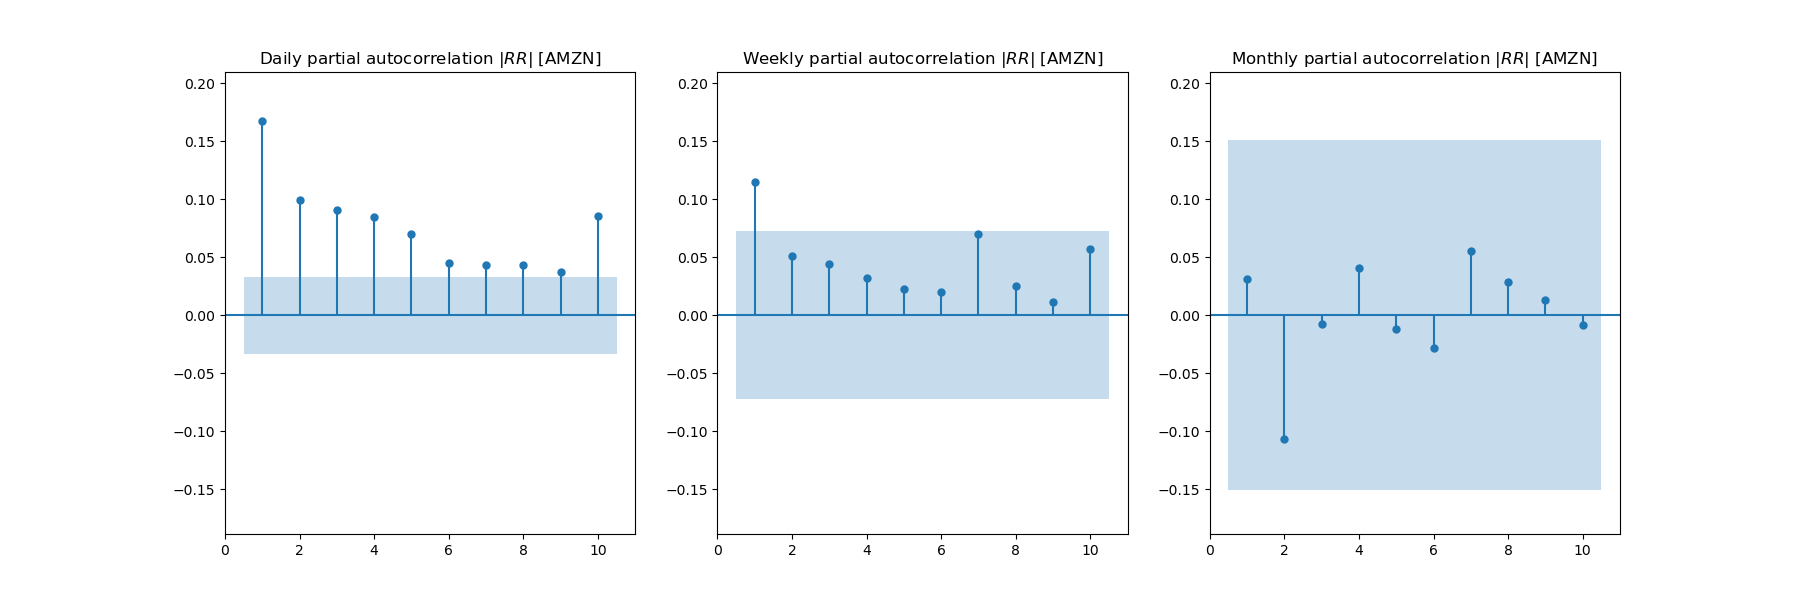
\includegraphics[width=0.8\linewidth]{images/partial_autocorrelation_abs_AMZN.png}
	\end{minipage}
\end{frame}

\subsection{Portafogli fattibili}
\begin{frame}{\subsecname}
	Vado ora a costruire empiricamente l'insieme dei portafogli fattibili andandoli a rappresentare come la coppia rendimento-rischio
	\[
		\biggl( 
			r(w_{1},...,w_{M}), \sigma^{2}(w_{1},...,w_{M})
		\biggr)= 
		\left( \sum_{m=1}^{M}w_{m}r_{m}, \sum_{l,m=1}^{M}w_{l}w_{m}\sigma_{l,m} \right)
	\]
	dove \( \sigma \) è la matrice varianza covarianza tra i tassi di rendimenti dei vari titoli. I pesi \( w_m \) sono stati generati da una distribuzione normale di media nulla per poi normalizzarli adeguatamente
	\[
		w_m = \frac{z_m}{\sum_{m=1}^{M} z_m}, \quad \forall m = 1, \dots, M,
	\]
\end{frame}

\begin{frame}{\subsecname}
	Generando casualmente 1000000 di portafogli, è interessante osservare come si distribuiscono secondo quanto previsto dalla teoria di Markowitz \\
	\vspace{-0.6cm}
	\begin{minipage}{0.49\textwidth}
		\centering
		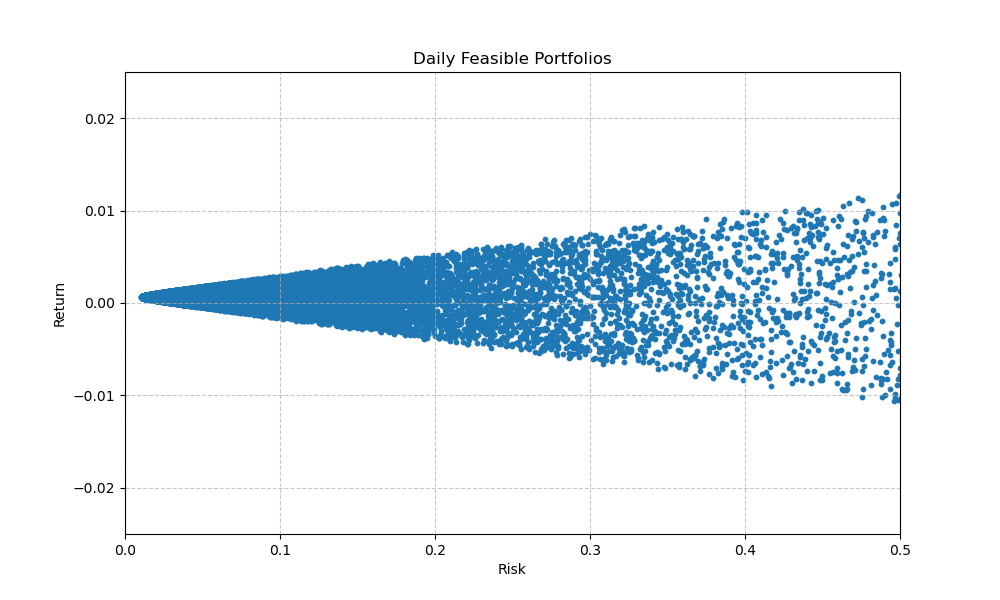
\includegraphics[width=1\linewidth]{images/Daily Feasible Portfolios.png}
	\end{minipage}
	\hfill
	\begin{minipage}{0.49\textwidth}
		\centering
		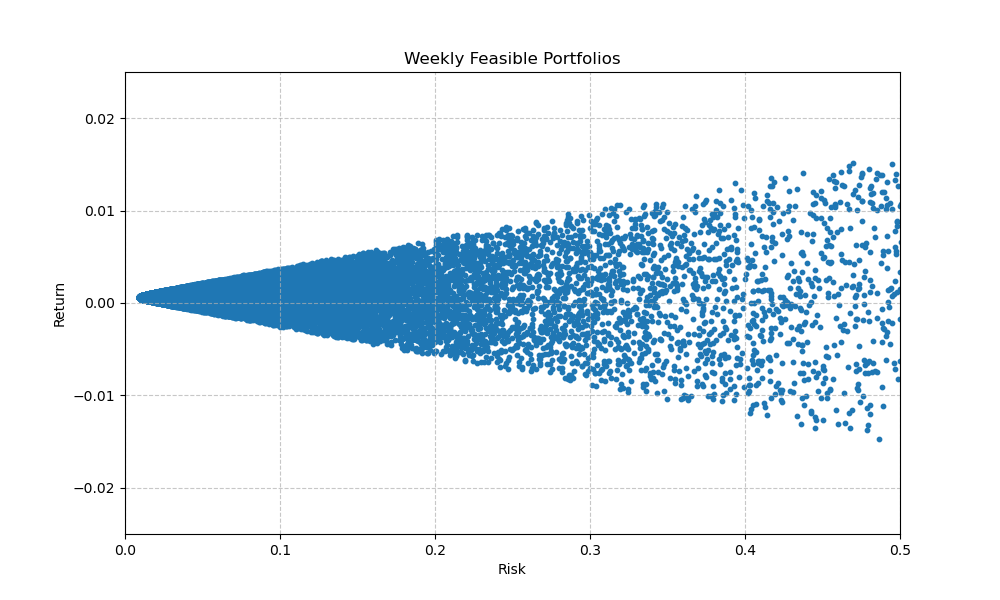
\includegraphics[width=1\linewidth]{images/Weekly Feasible Portfolios.png}
	\end{minipage}
	\vspace{0.13cm}
	\begin{center}
		\begin{minipage}{0.5\textwidth}
			\centering
			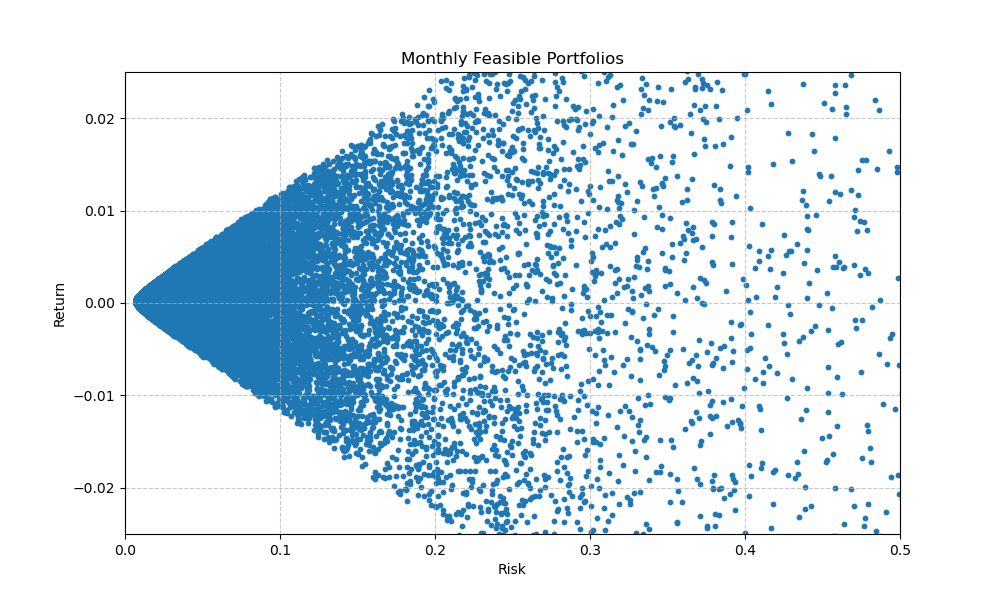
\includegraphics[width=0.95\linewidth]{images/Monthly Feasible Portfolios.png}
		\end{minipage}
	\end{center}
\end{frame}

\subsection{Frontiera efficiente}
\begin{frame}{\subsecname}
	A questo punto risolvendo il problema di ottimizzazione vincolata in cui per ogni rendimento cerco la combinazione di pesi che minimizza il rischio, ottengo la frontiera efficiente
	
	\begin{minipage}{0.29\textwidth}
		\[
		\begin{array}{ll}
			\text{Minimize:} & \sqrt{\mathbf{w}^T \mathbf{\Sigma} \mathbf{w}} \\
			\text{Subject to:} & \sum_{i=1}^{n} w_i = 1 \\
			& \mathbf{w}^T \mathbf{r} = r_t \\
			\end{array}
		\]
	\end{minipage}
	\hfill
	\begin{minipage}{0.62\textwidth}
		\centering
		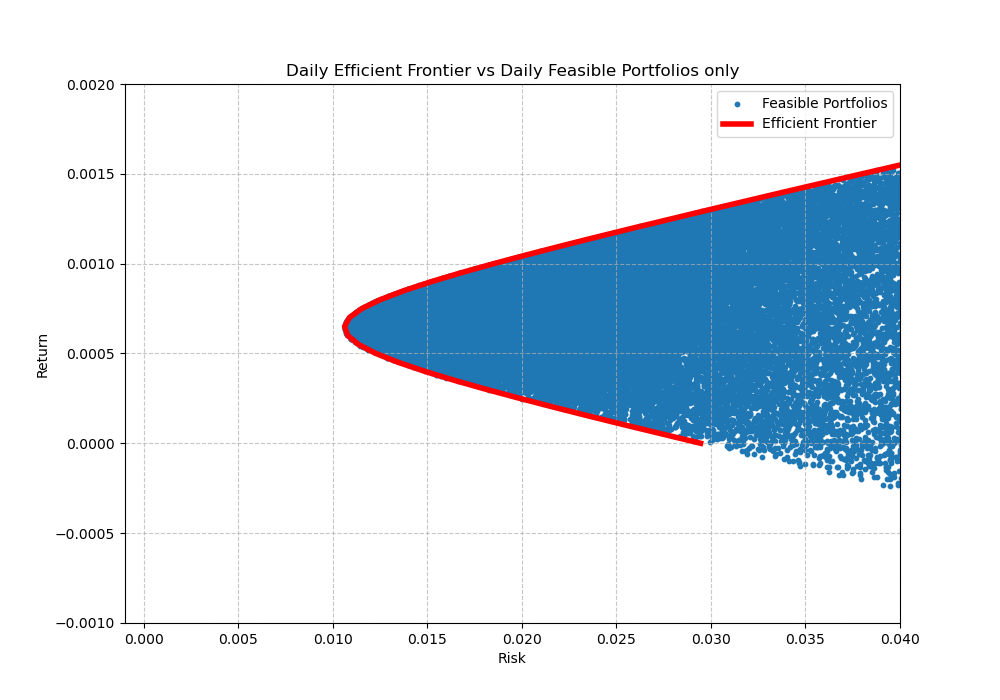
\includegraphics[width=1\linewidth]{images/Daily Efficient Frontier vs Daily Feasible Portfolios only.png}
	\end{minipage}
\end{frame}

\subsection{Rendimento privo di rischio}
\begin{frame}{\subsecname}
	L'inclusione di un rendimento privo di rischio consente di ottimizzare il rapporto rendimento-rischio, rivelando una relazione lineare tra volatilità e rendimento ottimali. 

	Come rendimento privo di rischio è stato considerato Real Interest Rate ad un mese messo a disposizone dalla \textbf{Federal Reserve Bank of St. Louis}. 

	\begin{itemize}
		\item Media sul periodo di riferimento
		\item Conversione in tasso giornaliero e settimanale
		\begin{itemize}
			\item \( r_{Weekly} = (1 + r_{Monthly})^\frac{1}{4} - 1 \)
			\item \( r_{Daily} = (1 + r_{Monthly})^\frac{1}{30} - 1 \)
		\end{itemize}
	\end{itemize}
\end{frame}

\begin{frame}{\subsecname}
	è possibile tracciare una retta tangente con il portafoglio tangente, ovvero il portafoglio che massimizza il rapporto rendimento-rischio. \\
	\vspace{-0.6cm}
	\begin{center}
		\begin{minipage}{0.8\textwidth}
			\centering
			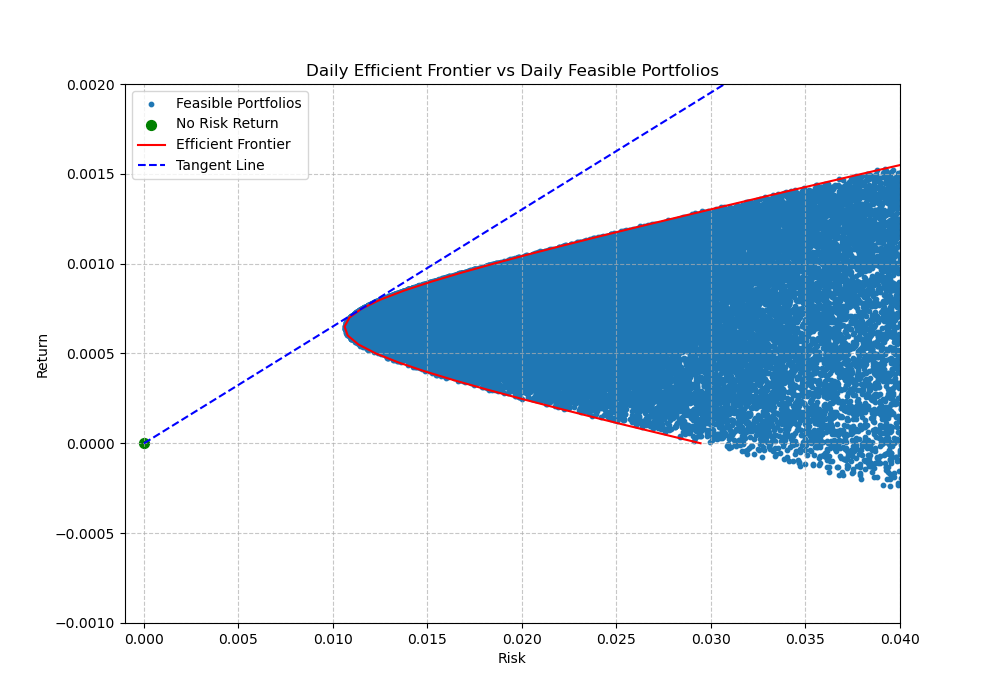
\includegraphics[width=1\linewidth]{images/Daily Efficient Frontier vs Daily Feasible Portfolios.png}
		\end{minipage}
	\end{center}
\end{frame}

\subsection{Portafoglio Tangente}
\begin{frame}{\subsecname}
	A questo punto è interessante verificare empiricamente che i possibili portafogli composti da titoli azionari e un titolo privo di rischio si posizonino effettivamente al di sotto della retta tangente. 
	\vspace{-0.6cm}
	\begin{minipage}{0.65\textwidth}
		\centering
		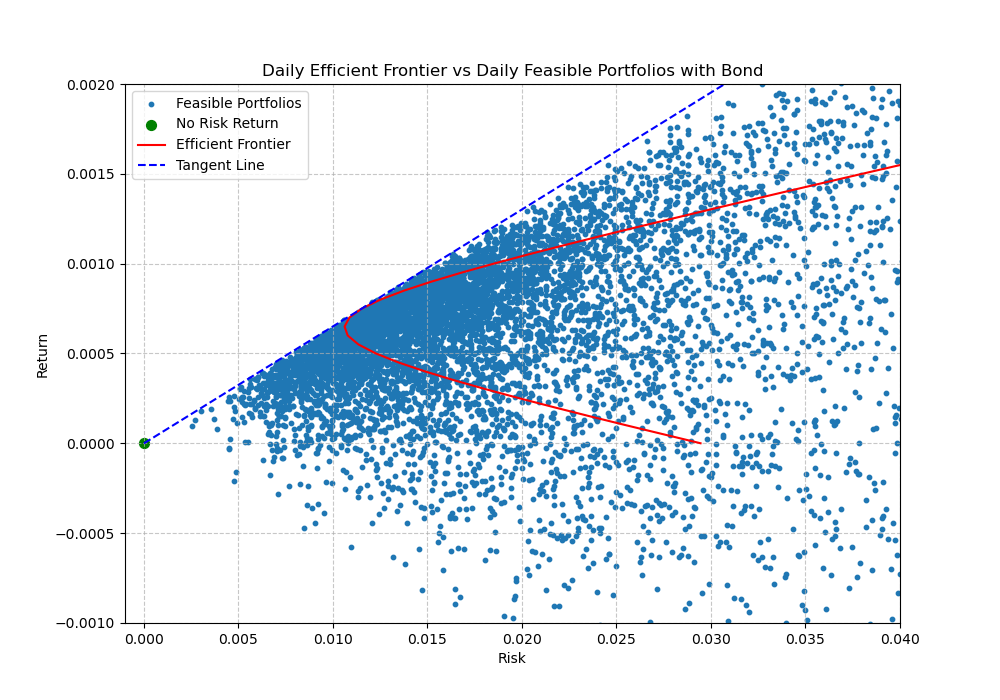
\includegraphics[width=1\linewidth]{images/Daily Efficient Frontier vs Daily Feasible Portfolios with Bond.png}
	\end{minipage}
	\hfill
	\begin{minipage}{0.30\textwidth}
		\centering
		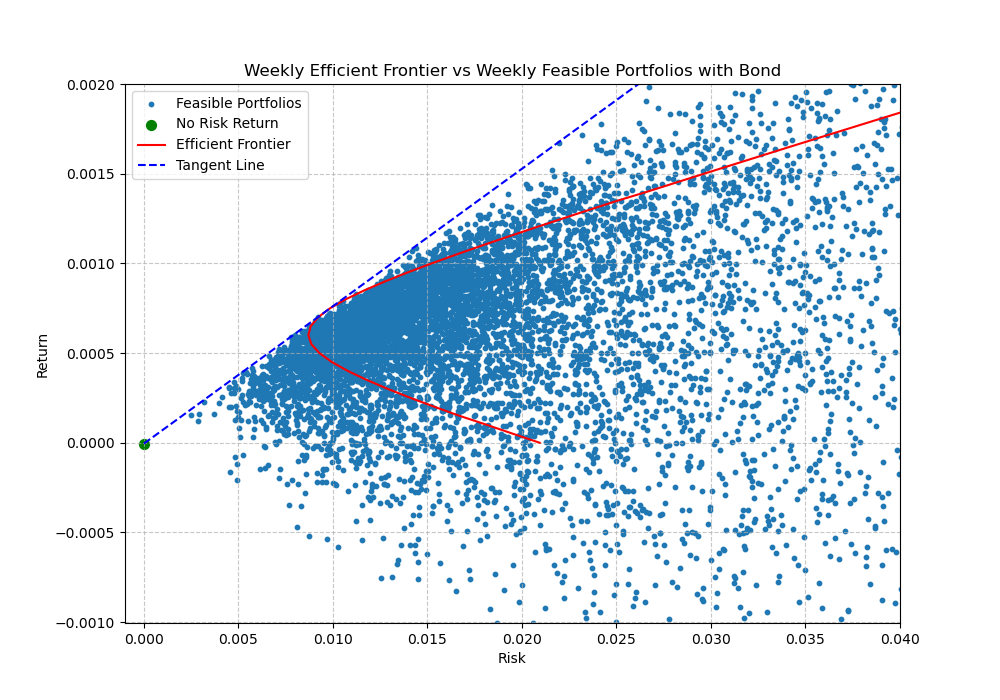
\includegraphics[width=1\linewidth]{images/Weekly Efficient Frontier vs Weekly Feasible Portfolios with Bond.png}
		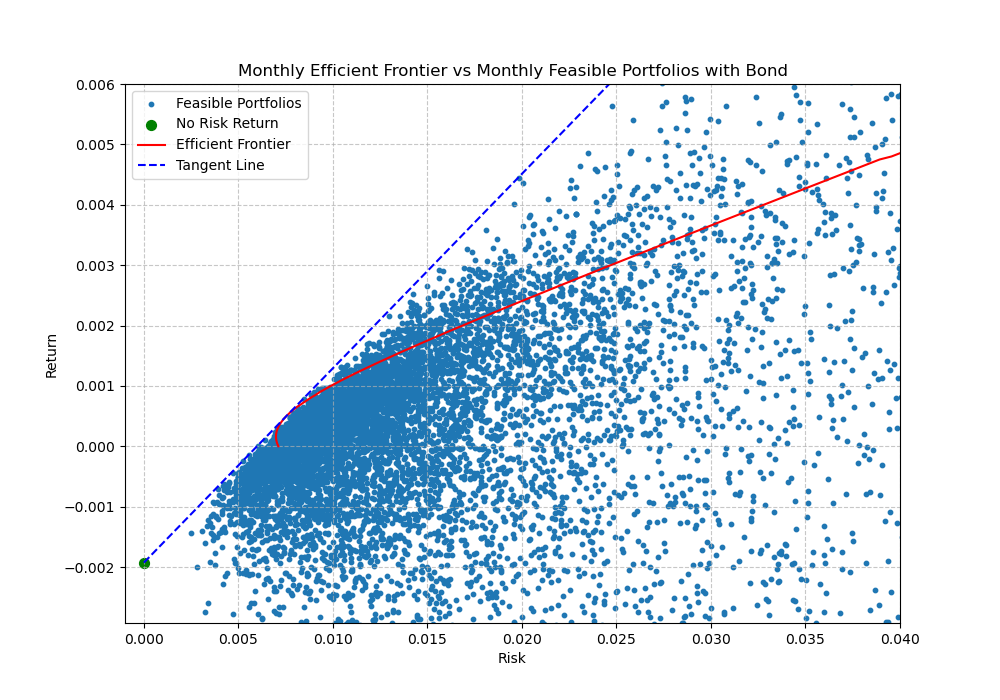
\includegraphics[width=0.95\linewidth]{images/Monthly Efficient Frontier vs Monthly Feasible Portfolios with Bond.png}
	\end{minipage}
\end{frame}

\section{CAPM}

\subsection{Capital Market Line}
\begin{frame}{\subsecname}
	La capital market line è una retta che collega il rendimento privo di rischio con il portafoglio tangente.
	I portafogli sulla capital market line sono una combinazione lineare tra il portafoglio tangente e il titolo privo di rischio. Dove il rendimento atteso del portafoglio è dato da
	\[
		r_a = \alpha \overline{r}_T + (1 - \alpha) r_0
	\]

	e il rischio assegnato del portafoglio è data da
	\[
		\sigma_a^2 = \alpha^2 \sigma_T^2 
	\]
\end{frame}

\begin{frame}{\subsecname}
	Andando a variare \(\alpha\) in è possibile notare come si dispongono i portafogli sulla retta. \\
	\vspace{-0.6cm}
	\begin{minipage}{0.65\textwidth}
		\centering
		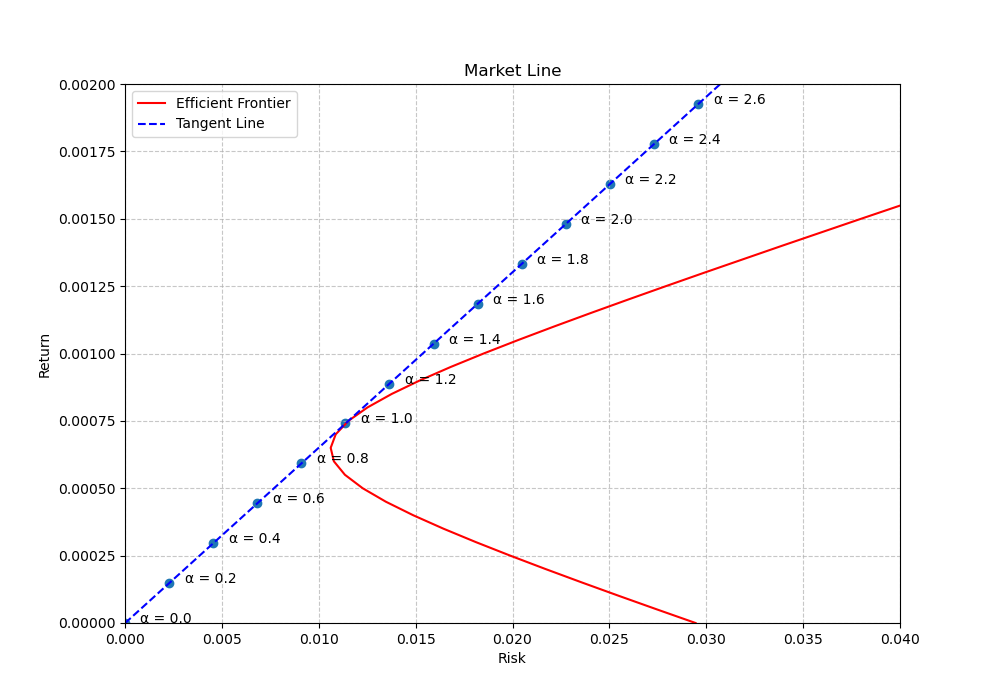
\includegraphics[width=1\linewidth]{images/Daily2.png}
	\end{minipage}
	\hfill
	\begin{minipage}{0.30\textwidth}
		\centering
		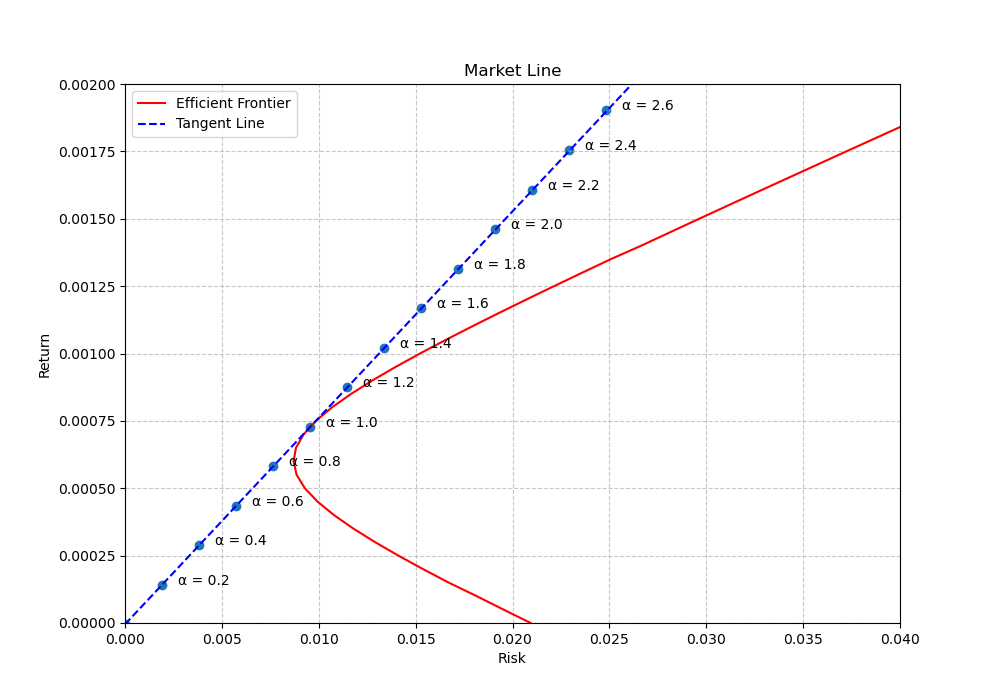
\includegraphics[width=1\linewidth]{images/Weekly2.png}
		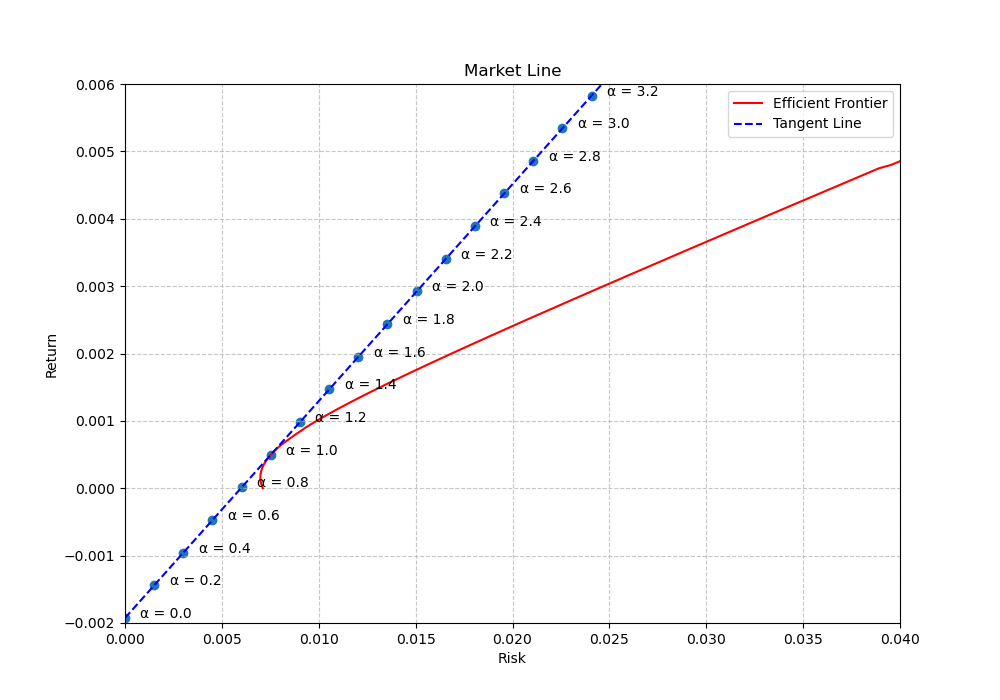
\includegraphics[width=0.95\linewidth]{images/Monthly2.png}
	\end{minipage} \\ \\ \\
	Quando \(\alpha>1\), significa che bisogna vendere allo scoperto dei bond (prendere in prestito dei soldi) per investirli nel portafoglio tangente.
\end{frame}

\subsection{Test CAPM hypotesys}
\begin{frame}{\subsecname}
	Secondo il CAPM il portafoglio tangente coincide con il portafoglio di mercato, ossia con il portafoglio
i cui pesi sono dati dalla capitalizzazione relativa dei titoli che compongono il mercato in rapporto alla
capitalizzazione dell'intero mercato. \\

Ipotizzando un mercato composto solo dai 5 titoli considerati, possiamo verificare empiricamente che il portafoglio tangente coincida con il portafoglio di mercato scegliendo i pesi con
\[
w_m = \frac{K_m}{K}
\]

dove \(K_m\) è la capitalizzazione di mercato media del titolo \(m\) nel periodo considerato e \(K = \sum_{m=1}^{M} K_m\)
\end{frame}

\begin{frame}{\subsecname}
	Ho inserito anche un ulteriore portafoglio, il portafoglio equamente pesato come benchmark aggiuntivo. \\ \\
	In questo caso i pesi sono dati da
\[
w_m = \frac{1}{M}
\]
\end{frame}

\begin{frame}{\subsecname}
	Nel caso giornaliero il portafoglio tangente coincide quasi perfettamente sia con il portafoglio di mercato che con quello equamente pesato
	\begin{center}
		\begin{minipage}{0.8\textwidth}
			\centering
			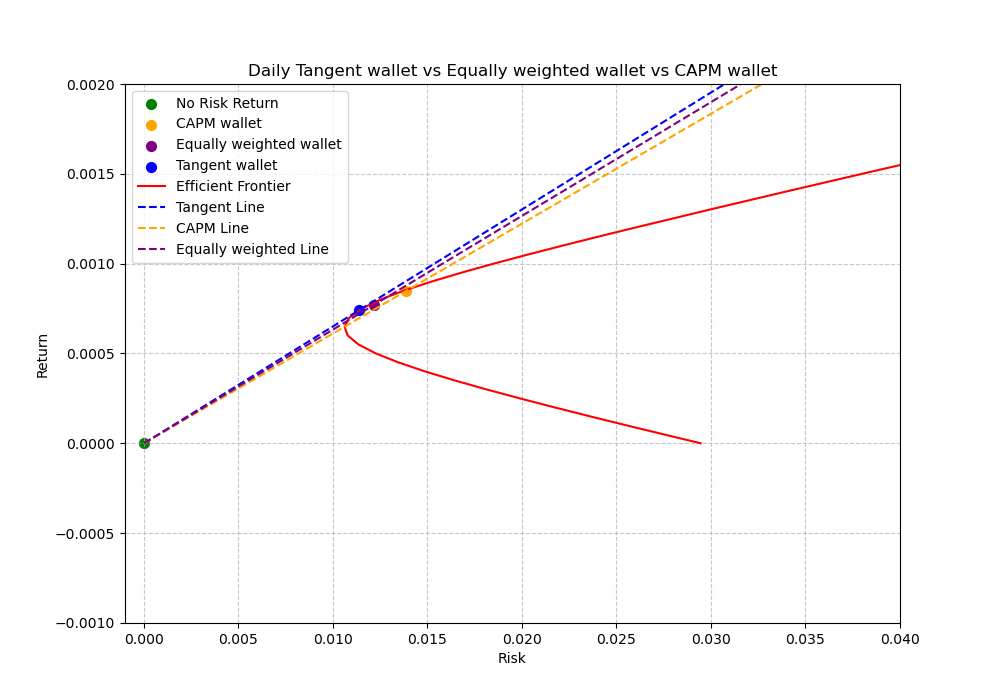
\includegraphics[width=1\linewidth]{images/Daily Tangent wallet vs Equally weighted wallet vs CAPM wallet.png}
		\end{minipage}
	\end{center}
\end{frame}

\begin{frame}{\subsecname}
	Nei casi settimanale e mensile invece c'è una leggera discrepanza tra il portafoglio tangente e il portafoglio di mercato. 
	\begin{center}
		\begin{minipage}{0.49\textwidth}
			\centering
			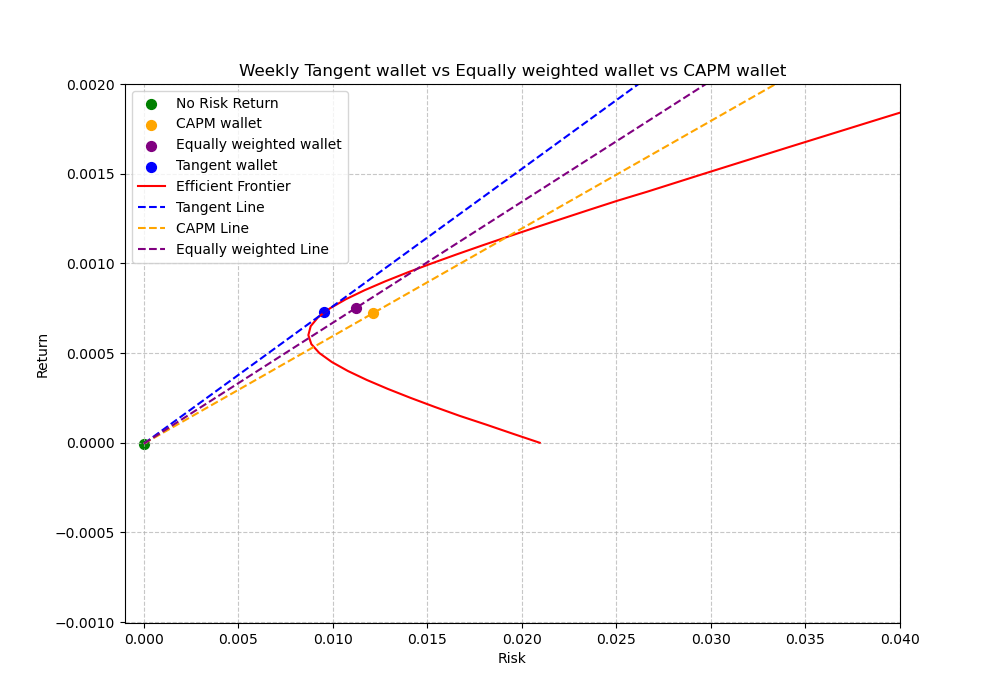
\includegraphics[width=1\linewidth]{images/Weekly Tangent wallet vs Equally weighted wallet vs CAPM wallet.png}
		\end{minipage}
		\begin{minipage}{0.49\textwidth}
			\centering
			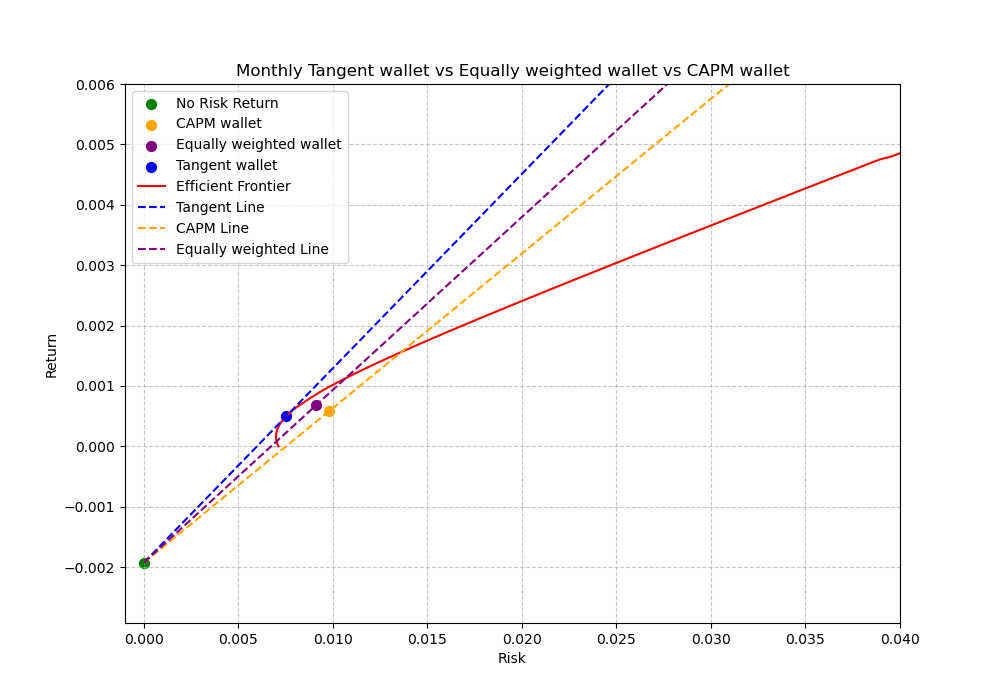
\includegraphics[width=1\linewidth]{images/Monthly Tangent wallet vs Equally weighted wallet vs CAPM wallet.png}
		\end{minipage}
	\end{center}

	Tuttavia il portafoglio equamente pesato si posiziona sempre un po' più vicino al portafoglio tangente
\end{frame}

\section{Conclusioni}

\begin{frame}{Conclusioni}
	\begin{itemize}
		\item All'aumentare dell'orizzonte temporale, i tassi di rendimento sembrano diventare sempre più stazionari.
		\begin{itemize}
			\item Servirebbero ulteriori test statistici per confermare questa ipotesi
		\end{itemize}
		\item I risultati empirici sembrano confermare la validità del modello di Markowitz
		\item Uguaglianza tra portafoglio tangente e portafoglio di mercato
		\begin{itemize}
			\item Sembra esserci una discrepanza possibilmente dovuta ai pochi titoli presi in considerazione
			\item Il portafoglio equamente pesato come portafoglio di mercato sembra una ipotesi plausibile, ma da validare con ulteriori test e considerazioni teoriche.
		\end{itemize}
	\end{itemize}	
\end{frame}
\begin{frame}
	\frametitle{Grazie per l'attenzione!}
	\begin{Huge}
		Domande?
	\end{Huge} 
	\\ \\
	Il codice è disponibile al seguente repository: \url{https://github.com/LucaFalasca/FinancialMarketAnalysis}
	\\ \\
	Grazie a tutti!
	
\end{frame}


\end{document}
